\section{Технический проект}

\subsection{Общие сведения о программно-информационной системе}

Полное наименование системы: Веб-приложение <<Социомаркет для владельцев домашних животных>>.

Краткое обозначение системы: <<Социомаркет>>.

Описание системы: Система <<Социомаркет>> предназначена для владельцев домашних животных, предоставляя им платформу для поиска и предложения различных услуг и товаров для животных. Система создана для облегчения доступа к широкому спектру услуг, от ветеринарной помощи до груминга и других товаров для животных.

Условия эксплуатации: <<Социомаркет>> предназначена для использования в нормальных условиях работы, доступна через веб-браузеры на персональных компьютерах и мобильных устройствах.

Архитектура системы: Программное обеспечение основано на клиент-серверной архитектуре, используя современные технологии веб-разработки, включая .NET Core для серверной части и Angular для клиентской части. Система поддерживает REST API для обеспечения взаимодействия между клиентом и сервером и использует базу данных PostgreSQL.

Технологии и инструменты: В разработке использовались Angular, HTML, JavaScript, SCSS для клиентской части, а также .NET Core и Entity Framework Core для серверной части. Для управления данными использовалась технология ORM (Object-Relational Mapping).

Особенности системы:
\begin{itemize}
    \item возможность авторизации для пользователей и поставщиков услуг;
    \item разработка удобного интерфейса для поиска продуктов (товаров и услуг);
    \item возможность управления карточками услуг и товаров для поставщиков.
\end{itemize}

\subsection{Обоснование выбора технологий проектирования}
\subsubsection{.NET Core}
Выбор .NET Core для серверной разработки обосновывается его производительностью, масштабируемостью и кросс-платформенностью, а также поддержкой работы с админ-панелью <<из коробки>>, что является важным фактором в современной разработке программного обеспечения \cite{mark_price}.
Начиная с версии .NET core 6.0, которая была выбрана для разработки, поддерживается работа с админ-панелью <<из коробки>>, что позволяет сэкономить ресурсы на разработки панели администратора.

\subsubsection{Entity Framework Core}
Entity Framework Core является ORM (Object-Relational Mapping) для .NET Core. Он позволяет работать с базами данных, используя объектно-ориентированный подход \cite{grinchenko}. Entity Framework Core позволяет работать с различными СУБД, в том числе с PostgreSQL, которая была выбрана для разработки. EF Core предоставляет удобные и мощные инструменты для разработки приложений, использующих CRUD подход.

\subsubsection{PostgreSQL}
Выбор PostgreSQL в качестве системы управления базами данных был обусловлен её высокой надежностью, поддержкой продвинутых SQL-функций и совместимостью с EF Core. PostgreSQL предлагает удобные функции для разработчиков, такие как JSON/JSONB поддержка, хранение процедур и триггеры, что делает её идеальной для комплексных приложений, требующих масштабируемости и гибкости. К тому же, PostgreSQL обладает мощными средствами для работы с большими объемами данных и комплексными запросами, что критично для обеспечения высокой производительности приложения.

\subsubsection{Angular}
Angular, выбранный для Frontend разработки, предоставляет строгую и требовательную архитектуру, что делает его идеальным инструментом для создания сложных и масштабируемых приложений.

Эффективность Angular в разработке интерактивных интерфейсов и легкость интеграции с REST API достигается с помощью сервиса HttpService, входящего в состав модуля AngularCoreModule.

Angular предоставляет возможность писать код на TypeScript, что упрощает разработку и поддержку приложения и обеспечивает более строгую реализацию принципов ООП в клиенской части приложения.

Еще одним значимым преимуществом выбранного фреймворка для Frontend разработки Angular, является его скорость и легкость интеграции с библиотекой для применения методик функционального и реактивного программирования -\- RxJs \cite{rxjs}.

Внедрение современных методик функционального и реактивного программирования с помощью библиотеки RxJs обусловлено тем, что помимо логики, выполняемой серверной частью приложения, которая берет на себя выполнение запросов к базе данных, также было необходимо разработать значительный объем логики в клиентской части приложения.

Такая логика включает как небольшие процедуры для обработки событий форм, кнопок и других элементов пользовательского интерфейста, так и функции-обработчики или функции-мапперы, которые могут выполнять изменения объекта внутри потока данных, без доступа к внешней данным вне этой функции. Инкапсуляция данных внутри функций-мапперов является наилучшим подходом при работе с данными, который клиентское приложение принимает от серверной части приложения.

Стоит заметить, что язык программирование JavaScript предоставляет механизм инкапсуляции данных, созданных внутри функций. Такой механизм изоляции данных называется <<Замыкание>>. Ключевое отличие в том, что <<Замыкание>> препятствует утечке локальных данных созданных внутри функции, тогда как специализированные функции RxJs предотвращают проникновение внутрь функции любых данных приложения за пределами этой функции, в том числе и глобальных, кроме тех, что были умышленно переданы в эту функцию в качестве ее параметров \cite{rxjs}.

\subsection{Проектирование пользовательского интерфейса}

На основании требований к пользовательскому интерфейсу, представленных в пункте 2.3 технического задания, был разработан графический интерфейс мобильного приложения, используя Angular с применением HTML, JavaScript и SCSS \cite{cssspecs}. Этот процесс подчеркивает важность интуитивно понятного и эффективного взаимодействия с пользователем \cite{kumskova}.

Разработанный интерфейс ориентирован на обеспечение легкости в использовании и интуитивного понимания функционала приложения, предоставляя пользователю гладкое и эффективное взаимодействие с приложением.

Легкодоступность для понимания всех элементов пользовательского интерфейса также способствует эффективному ручному тестированию интерфейса, что было использовано и реализовано в рамках данной работы.

\begin{enumerate}
    \item \textbf{Поиск}: Реализация функции поиска на основе поля \textit{ProductName} из класса \textit{Product}, \textit{Price}, \textit{Weight}, и \textit{ProductGroupId} класса \textit{Product};
    \item \textbf{Отображение результатов поиска}: Эффективное представление списка товаров, включая \textit{ImageUrl}, \textit{ProductName}, информацию о \textit{Category} и \textit{Price};
    \item \textbf{Детали товара}: Дополнительная информация о товаре, включая его \textit{Category} и \textit{Weight};
    \item \textbf{Навигация по приложению}: Элементы навигации, такие как кнопка возврата к началу списка и индикаторы категорий.
\end{enumerate}

\begin{figure}[h!]
    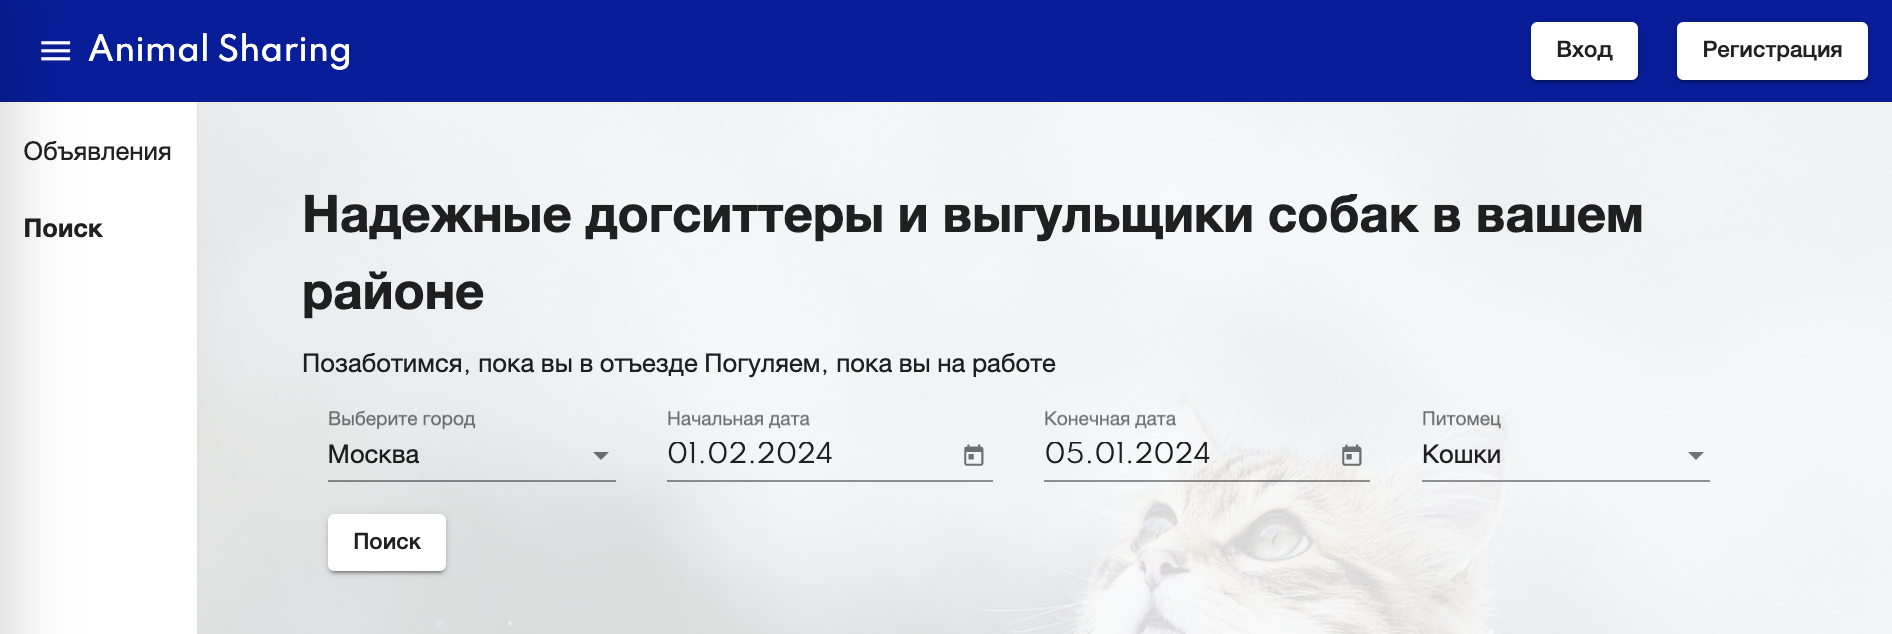
\includegraphics[width=0.82\linewidth]{interface-search}
    \caption{модели интерфейса <<Поиск>> и <<Навигация по приложению>>}
    \label{fig:search}
\end{figure}

Процесс регистрации пользователя в приложении максимально упрощен и включает следующие шаги:
\begin{enumerate}
    \item Пользователь выбирает опцию <<Регистрация>> на главном экране;
    \item Заполняются основные поля: электронная почта, имя пользователя и пароль;
    \item Пользователь должен подтвердить свой адрес электронной почты через полученное письмо со ссылкой для подтверждения;
    \item После подтверждения электронной почты, пользователь может ввести дополнительную информацию в свой профиль: фотографию, контактные данные и предпочтения в приложении;
    \item На последнем этапе пользователь принимает условия пользования и политику конфиденциальности, после чего регистрация завершается.
\end{enumerate}

Регистрация дог-ситтеров предполагает прохождение дополнительных этапов для верификации и предоставления информации о предоставляемых услугах:
\begin{enumerate}
    \item Потенциальный дог-ситтер начинает регистрацию с выбора соответствующего пункта в приложении;
    \item Вводятся личные данные, включая полное имя, адрес проживания и номер телефона;
    \item Запрашивается информация о предыдущем опыте работы с животными и наличии соответствующих рекомендаций;
    \item Дог-ситтер должен пройти онлайн-курс по уходу за животными и предоставить сертификат о его окончании;
    \item Предоставляется информация об услугах, включая доступные даты и временные рамки, а также устанавливаются тарифы;
    \item Профиль дог-ситтера отправляется на проверку. После одобрения администрацией профиль становится доступным для поиска и выбора пользователями.
\end{enumerate}


\begin{figure}[h!]
    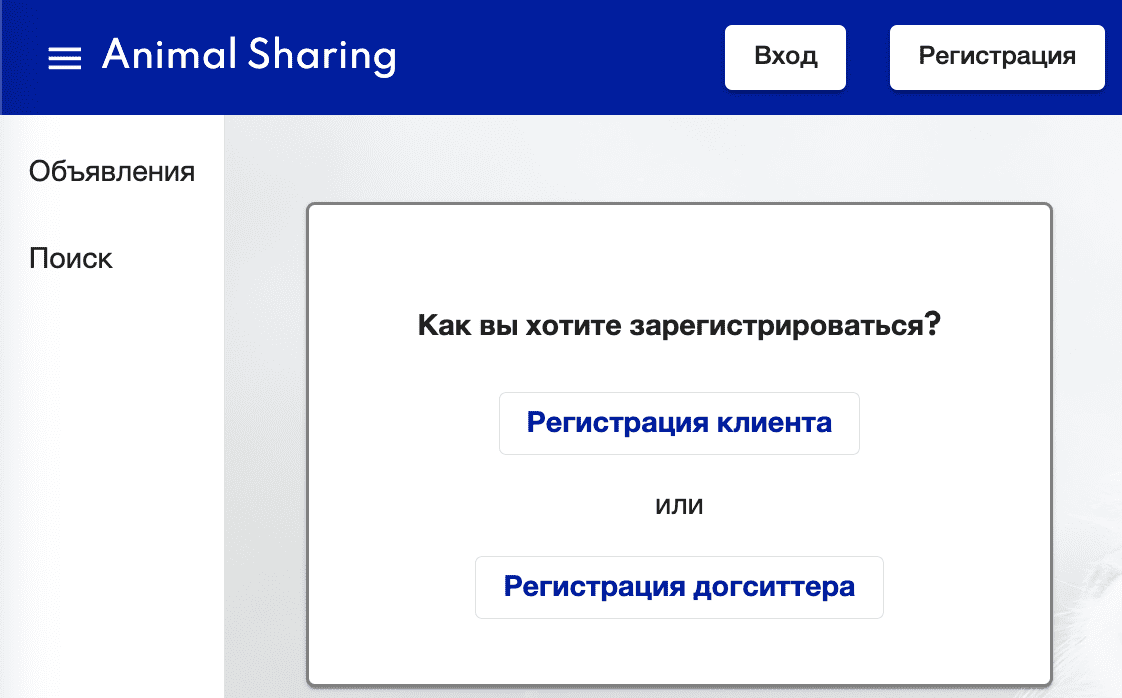
\includegraphics[width=0.82\linewidth]{interface-register}
    \caption{Модели интерфейса регистрации <<Пользователя>> и <<Дог-ситтера>>}
    \label{fig:register}
\end{figure}

\subsection{Диаграмма размещения}

Диаграмма размещения, отображаемая на рисунке \ref{place:image}, является фундаментальным инструментом для иллюстрации взаимосвязей между программными и аппаратными компонентами системы. Этот элемент визуализации служит для акцентирования значимости стратегического планирования в процессе разработки распределенных систем. Детальное и глубокое понимание этих взаимосвязей критически важно для успешного создания и функционирования распределенных информационных систем\cite{makni}. Каждый компонент системы, будь то программный или аппаратный, играет важную роль в обеспечении её общей эффективности и надежности. Подход, основанный на стратегическом планировании, способствует оптимизации этих взаимодействий и повышает вероятность успешной реализации и эксплуатации системы в целом.

\begin{figure}[ht]
\center{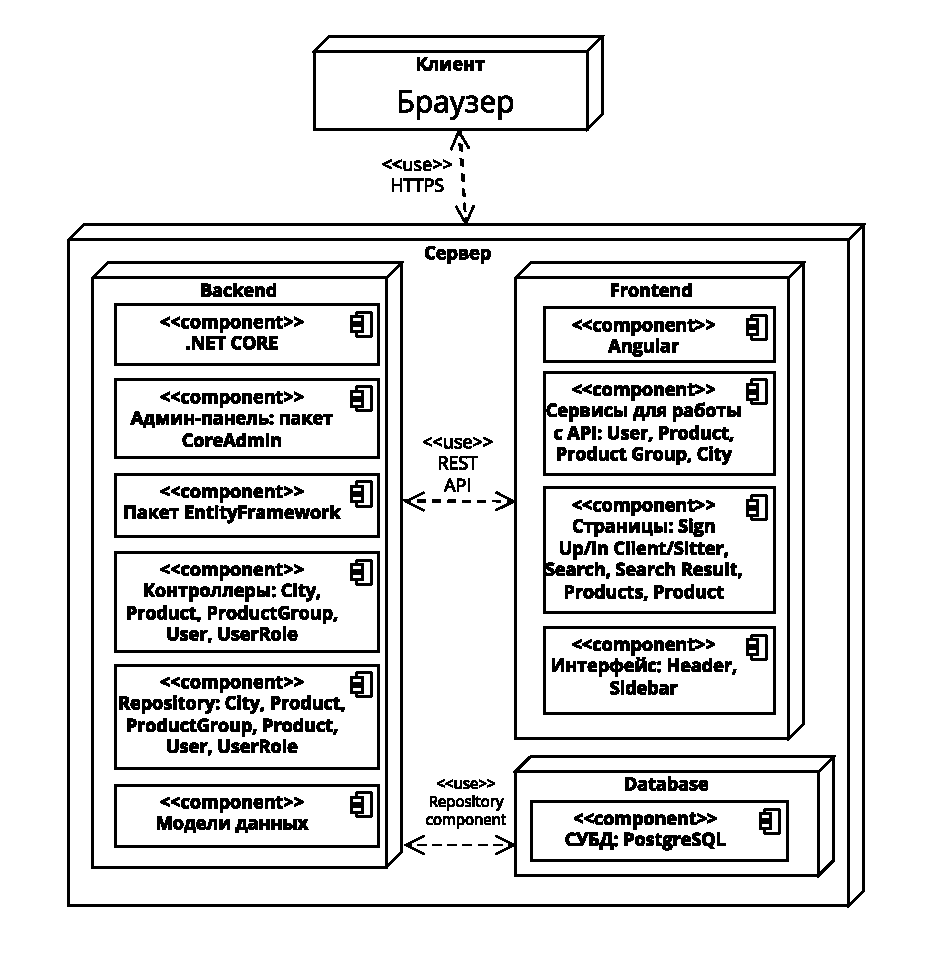
\includegraphics[width=1\linewidth]{client-server.eps}}
\caption{Диаграмма размещения}
\label{place:image}
\end{figure}

Диаграмма размещения является хорошим средством для показа маршрутов перемещения объектов и компонентов в распределенной системе.

Помимо данных о физическом размещении клиентской, серверной частей приложения, СУБД, на диаграмме размещения содержатся упоминания технологий и программных модулей, используемых для взаимодействия этих компонентов внутри клиент-серверной архитектуры веб-приложения.

\subsection{Описание архитектуры приложения}

Архитектура приложения, реализованная в рамках текущего исследования, базируется на модели MVC (Model-View-Controller) \cite{kofman}. Этот паттерн был избран благодаря его выдающейся способности к эффективному разделению функциональных обязанностей между структурными компонентами системы, а также способствованию упрощению процессов разработки и тестирования.

Паттерн MVC реализован следующим образом:

\begin{enumerate}
    \item Модель (Model) и Контроллер (Controller): Обе эти компоненты были разработаны на платформе .NET, обеспечивая управление бизнес-логикой и обработку данных, а также связь между пользовательским интерфейсом и базой данных;
    \item Представление (View): Реализовано через фронтенд, использующий фреймворк Angular, отвечающий за визуализацию информации и интерактивное взаимодействие с пользователем.
\end{enumerate}

Ключевым аспектом в управлении данными является использование системы управления базами данных PostgreSQL \cite{kofman}. Этот выбор был обусловлен высокой надежностью PostgreSQL, её превосходной производительностью и гибкостью в обработке сложных запросов, что имеет критическое значение для эффективного функционирования бэкенда.

Применение архитектуры MVC принесло следующие ключевые преимущества:

\begin{itemize}
  \item четкое Разделение Обязанностей: Эффективное разграничение между пользовательским интерфейсом (Angular) и серверной логикой (.NET) значительно упрощает процесс разработки и последующей поддержки системы \cite{kofman};
  \item гибкость и Масштабируемость: Благодаря MVC, архитектура приложения легко адаптируется и масштабируется, что позволяет разработчикам модифицировать или расширять отдельные части системы без влияния на другие;
  \item упрощение Тестирования: Независимость компонентов архитектуры MVC облегчает процедуру тестирования, позволяя проводить её для каждого элемента в отдельности \cite{kofman}.
\end{itemize}

Итоговая архитектура, базирующаяся на MVC в сочетании с Angular для фронтенда, .NET для бэкенда и PostgreSQL для управления данными, обеспечивает создание надежной, гибкой и масштабируемой системы. Данная архитектура представляет собой устойчивую основу для разработки современных программных решений, способных соответствовать как нынешним, так и будущим техническим и функциональным требованиям \cite{kofman}.
